
\chapter{Discussion}

\acresetall


\section{Humanly Perceived Improvement vs. Machine Performance}

The aim of conducting research into existing data was to determine,
at a basic level, the correlation between \ac{HR} and \ac{MR}.


\subsection{Investigating Existing Data}

Results from conducting a direct comparison between \ac{PESQ} and
\ac{PRR} results were given in \figref{Direct-PESQ-PRR}. These results
show a general, positive correlation between \ac{PESQ} improvement
and \ac{PRR} improvement, and by extension between \ac{HR} and \ac{MR}.
The level of correlation appears to be relatively low, however comparison
with \figref{litResCorr} indicates the such levels of correlation
are expected. Indeed, similar correlations are observed between \ac{PESQ}
and \ac{MOS} results, which are both \ac{HR} measures.

\figref{litResCorr} Also indicates a very high correlation between
the raw \ac{PESQ} result and \ac{PRR}.

A number of further observations were drawn from \figref{Direct-PESQ-PRR},
and are highlighted in \Cref{fig:direct-klt-mband,fig:direct-klt-pklt,fig:direct-pklt-logmmse-spu-4,fig:direct-highcorr}.

Despite the high correlation between \ac{PESQ} and \ac{PRR} observed,
there is still evidence to show that algorithms' performances vary
depending on the performance measure used. For example, highlighted
in \figref{direct-klt-mband} are two algorithms, the \ac{KLT} method
and the \ac{MBAND} method, that exhibited similar performances when
evaluated by \ac{PRR}, a machine measure. However, when evaluated
by a human perceptual method, \ac{PESQ}, the \ac{KLT} method clearly
performed better. In fact, the \ac{KLT} method exhibited one of the
best performances seen on the \ac{PESQ} scale, whereas the \ac{MBAND}
method was the worst performer on this scale, exhibiting loss in perceptual
quality, as indicated by the negative performance.

\begin{figure}[h]
\noindent \begin{centering}
\includegraphics[width=0.8\textwidth]{fig/R/dir/lit/KLT-MBAND/HumanMachineAllLM}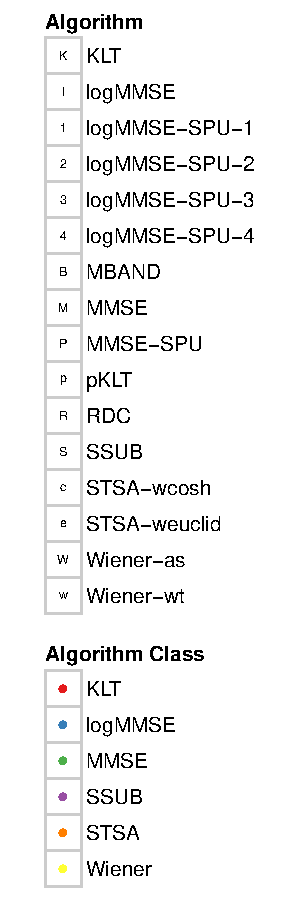
\includegraphics[width=0.2\textwidth]{fig/R/dir/lit/HumanMachineAllLegend}
\par\end{centering}

\protect\caption{\label{fig:direct-klt-mband}Direct comparison of \acs{PESQ} vs.
\acs{PRR} highlighting \acs{KLT} and \acs{MBAND}}
\end{figure}


\figref{direct-klt-pklt} shows the \ac{PESQ} vs. \ac{PRR} improvement
with the \ac{KLT} and \ac{pKLT} algorithm performances highlighted.
This was noted as an example of two very similar algorithms, with
varying performance between \ac{HR} and \ac{MR} results. The \ac{KLT}
results exhibited better performance for a human listener, as the
points laid higher on the y-axis, whereas the \ac{pKLT} results exhibited
better performance for a machine recogniser, as the points laid higher
on the x-axis.

\begin{figure}[p]
\noindent \begin{centering}
\includegraphics[width=0.8\textwidth,height=0.25\textheight,keepaspectratio]{fig/R/dir/lit/KLT-pKLT/HumanMachineAllLM}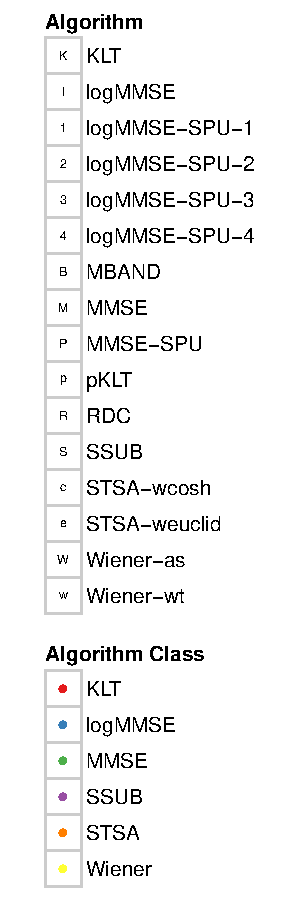
\includegraphics[width=0.2\textwidth,height=0.25\textheight,keepaspectratio]{fig/R/dir/lit/HumanMachineAllLegend}
\par\end{centering}

\protect\caption{\label{fig:direct-klt-pklt}Direct comparison of \acs{PESQ} vs. \acs{PRR}
highlighting \acs{KLT} and \acs{pKLT}}
\end{figure}


Such results support the proposition that some algorithms are inherently
suited either towards human or machine listeners. However, this shows
that such distinction is not necessarily related to the algorithm
class, since the \ac{KLT} and \ac{pKLT} algorithms belonged to the
same \ac{KLT} class, but produced different results.

The \ac{pKLT} and \ac{logMMSE-SPU-4} algorithms were observed to
show reasonable improvement in \ac{PRR} as the \ac{SNR} increased,
but little to no improvement in \ac{PESQ}. This is highlighted in
\figref{direct-pklt-logmmse-spu-4}, and is apparent by the near-zero
gradient. These algorithms likely introduce distortions into the signal
in the process of enhancement that the \ac{ASR} algorithm was immune
to, however would be distracting to a human and therefore performed
badly under the \ac{PESQ} evaluation.

\begin{figure}[p]
\noindent \begin{centering}
\includegraphics[width=0.8\textwidth,height=0.25\textheight,keepaspectratio]{fig/R/dir/lit/pKLT-logMMSE-SPU-4/HumanMachineAllLM}
\par\end{centering}

\protect\caption{\label{fig:direct-pklt-logmmse-spu-4}Direct comparison of \acs{PESQ}
vs. \acs{PRR} highlighting \acs{logMMSE} \acs{SPU} and \acs{pKLT}}
\end{figure}


The final observation drawn from \figref{Direct-PESQ-PRR} is highlighted
in \figref{direct-highcorr}, which shows the \ac{MMSE-SPU}, \ac{STSA-wcosh},
\ac{STSA-weuclid} and \ac{logMMSE-SPU-3} algorithms. These algorithms
show a high, positive correlation with one another, as well as exhibiting
the best results measured for both \ac{PESQ} and \ac{PRR}. The evidence
suggests such a response is the ideal case, and that there exists
algorithms which are capable of performing well for both human and
machine recognisers.

\begin{figure}[p]
\noindent \begin{centering}
\includegraphics[width=0.8\textwidth,height=0.25\textheight,keepaspectratio]{fig/R/dir/lit/MMSE-SPU-STSA-wcosh-STSA-weuclid-logMMSE-SPU-3/HumanMachineAllLM}
\par\end{centering}

\protect\caption{\label{fig:direct-highcorr}\acs{STSA-wcosh}, \acs{STSA-weuclid}
and \acs{logMMSE-SPU-3}}
\end{figure}


Results found using the grouped comparison method, shown in \figref{Group-PESQ-PRR-LOESS}
indicated that the data could be approximated by a linear model. The
\ac{LOESS} fitted lines were, in most cases, approximately linear.
The results for Wiener algorithms were a notable exception, with a
non-linear variation, even when the outliers are ignored. Overall,
the \ac{LM} fit in \figref{Group-PESQ-PRR-LM} is accepted to be
accurate.

The grouped linear fittings also correlate well with the best performing
individual algorithms, those highlighted in \figref{direct-highcorr}.

{*}{*}\textit{Conclusion, at the moment, is looking to be that in
general there is a good correlation between human and machine listener
improvement, and that, therefore, there will likely be many algorithms
suited to both purposes. However, still to warn that algorithms should
be verified both ways, as one does not imply the other.}


\subsection{Independent Investigation into \acl{HR} and \acl{MR}}

An independent investigation was conducted in which a number of enhancement
algorithms were implemented. The enhanced waveforms were then analysed
using a number of enhancement methods, covering both \ac{HR} and
\ac{MR}. The goal was to determine the correlation between evaluation
measures.

A summary of the correlation between all measurements made is given
in \figref{my-Corr}. A number of interesting observations were drawn
from this summary to be further investigated.

Firstly, it was noted that in \figref{my-Corr}, the correlation between
\ac{PESQ} and the various \ac{MOS} measures was low. This was a
surprising results as it has generally been determined in literature
that the two correlate well \cite{Kitawaki2007,Rix2003,Rix2001},
albeit with some exceptions \cite{Liu2006}. It was also noted that
the ideal binary mask algorithms performed very poorly overall on
the subjective scales in \Cref{fig:my-MOS,fig:my-MOSle,fig:my-CMOS}.
Furthermore, ideal binary mask algorithms had a very high variation
in \ac{PESQ} performance in \figref{my-PESQ}. Therefore, it was
suspected these results may be adversely affecting the overall correlation
between \ac{PESQ} and \ac{MOS}.

It was found that when the ideal binary mask algorithm data was omitted
the correlation between the \ac{PESQ} and \ac{MOS} increased, as
demonstrated in \figref{my-pesq-mos}. This indicated there were specific
occurrences for which the relationship between \ac{PESQ} and \ac{MOS}
demonstrated in literature do not hold.

\begin{figure}[h]


\subfloat[With the ideal binary mask]{

\includegraphics[width=0.4\textwidth]{fig/R/pair/my/pesq-mos}

}\subfloat[Without the ideal binary mask]{

\includegraphics[width=0.4\textwidth]{fig/R/pair/my/pesq-mos_no-IDBM}

}\includegraphics[width=0.2\textwidth]{fig/R/pair/my/pesq-mos_leg}

\protect\caption{\label{fig:my-pesq-mos}Scatterplot of \acs{PESQ} vs. \ac{MOS} results}
\end{figure}


The \ac{MOS} evaluation measures had a strong correlation with one-another
in \figref{my-Corr}, all at approximately 90\%. This was expected
between similar measures. However, it was noted that the same was
not true for the \ac{PRR} measures, where the correlation between
the correctness and the accuracy was found to be in general significantly
negative.


\section{Assessing \acl{NMF} Algorithm Training}


\subsection{Investigating Training Requirements}

The investigation to investigate training was conducted on two recently
proposed \ac{NMF} algorithms of interest, an online \ac{BNMF} and
a supervised \ac{BNMF}.


\subsubsection*{General Performance}

The algorithm performance was poor on the supplied test data. It can
be seen in \figref{vary-train-pesq-imp} that in general the enhanced
algorithm performed worse than the dirty recording, by the fact that
the improvement scores are predominantly negative. The algorithms
produced similar patterns consistently across tests, indicating it
is unlikely results are randomised outliers.


\subsubsection*{Online \acl{BNMF}}

Before tests were performed, it was hypothesised that increasing the
number of utterances provided as training would allow the algorithm
to produce a better model, with more data to learn from. However,
the number of utterances provided for training of the online \ac{BNMF}
algorithm in \figref{vary-train-pesq} had no significant impact on
\ac{PESQ} performance. In fact, a slight negative correlation may
be noted, which is supported by results in \figref{train-req-corr}.
